\chapter{Embedded System}
\label{chap:embedded}
This chapter details the development of the embedded system necessary for controlling and actuating the hopper. It consists of two
major parts,
\begin{enumerate}
\item
Micro-controller and RF interface
\item
Inertial Measurement Unit (IMU)
\end{enumerate}

\section{Micro-controller}
The micro-controller chosen for this system is a Microchip dsPIC33F64MC804. It can run at 40 MIPS with an onboard flash memory of
64 KB along with a 16 KB SRAM. There are a host of integrated peripherals like Serial Peripheral Interface (SPI), UART, Analog to
Digital converter (ADC), Quadrature Encoder (QEI) and timers to generate Pulse Width Modulation (PWM) that can be used for motor
control.
Other major features provided with it are the Direct Memory Access controller (DMA) which can transfer memory from one peripheral
to other without CPU intervention and the high multiplexing of its IO pins. The latter enables almost all IO pins to be assigned
to any of the above mentioned peripherals (except analog pins) and greatly simplifies design. Pickit 2 is a programmer cum
debugger that had been ordered for programming the micro-controller.\\

XBee modules using the Zigbee protocol are used to form a wireless link with the embedded system on the hopper. The range of these
devices is quite sufficient for indoor uses (about 100 m). The interface on the micro-controller side is through UART and a custom
made FT232 module will be used to interface it with the base station to gather telemetry. A python module to grab and plot this 
telemetry from the virtual serial port of FT232 is in development.\\

The current development board contains one motor driver and its adjoining encoder port. The final module will contain two motor
drivers and encoder arrangements for the pinion and the reaction wheel motors.

\section{Inertial Measurement Unit (IMU)}

\subsection{Hardware}
We need to read the current pitch of the hopper for proper reorientation before every hop. This is done with the help of an IMU.
It consists of a two-axis accelerometer (ADIS 16201) and a single axis gyroscope (ADIS 16255). Both provide 14-bit signed readings
via the SPI interface with internal temperature bias compensation for the gyroscope. Using a digital sensor has benefits over
an analog output sensor because the ADC of the micro-controller can give a maximum resolution of only 12 bits as compared to the
14-bit reading given by these sensors.\\

The sensitivity of the gyroscope is $0.07326$ $^o/$s/LSB for the whole range of $\pm\;320$ $^o/$s with a noise of $0.48$ $^o/$s. The accelerometer has a sensitivity of 2.162 LSB/mg with a noise of 22 LSB. The accelerometer also consists of an
inclinometer to measure the angle with respect to the ground. However, it provides a sensitivity of only 10 LSB/deg. This
necessitates the need of onboard inverse tangent tables to get the pitch angle from accelerometer readings. The bandwidth of the
gyroscope is 50 Hz as compared to 2.25 kHz of the accelerometer. This severely limits the update rate of the filter and hence we
need a better gyroscope.

\subsection{Kalman Filter}
\begin{figure}[!h]
\centering
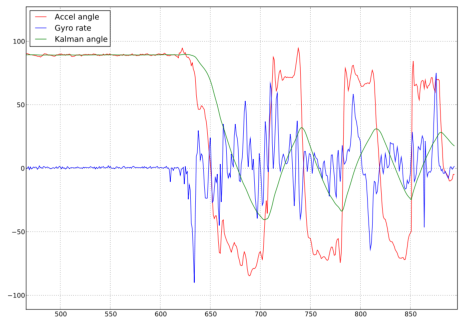
\includegraphics[scale=0.8]{fig/kalman_lowfreq.pdf}
\caption{Kalman filter : Low frequency input}
\label{fig:5_kalman_lowfreq}
\end{figure}
As shown in Fig. \ref{fig:5_kalman_lowfreq}, the readings of the gyroscope and the accelerometer are highly noisy and erratic even
in the situation of smooth movements of the IMU. This shows, that depending upon either of the two sensors is not good for
pitch estimation. Gyroscopes are high frequency sensors and accurately estimate the rate. However, they also show pronounced
variation of 
readings with time (gyro bias) and temperature (compensated to an extent). Accelerometers are good at low frequency
measurements. These do not suffer from a growing bias like the gyroscopes and can be used to correct the
readings estimated on the basis of gyroscope rate from time to time. We look at Kalman filter as a way to fuse these two sensors.\\

Various alternatives for filtering schemes exist and complementary filters are very widely used for fusing accelerometers and 
gyroscopes on IMUs. I decided to use a Kalman filter because the micro-controller can easily handle the computations
at usable update rates of about 20-50 Hz. This is one of the major reasons cited in literature for the use of complementary
filters over Kalman filters \cite{kalman1975}. It is also noted that for linear systems, there is little difference in the equations
of the two filters.\\

The equations for Kalman filter with a state vector $\bm{x} = [x_1\;\;x_2]^T = [\theta\;\;\dot{\theta}]^T$ are give below \cite{kalman_book}.\\

State equation :
\begin{equation}
\label{eqn:5_kalmanstate}
\bm{x}_{k+1} = \bm{A}\:\bm{x}_k + \bm{B}\:\bm{u}_k + \bm{w}_k
\end{equation}
Output equation :
\begin{equation}
\label{eqn:5_kalmanop}
y_{k+1} = \bm{C}\:\bm{x}_{k+1} + z_{k+1}
\end{equation}
Update equations :
\begin{equation}
\label{eqn:5_kalmanK}
\bm{K}_k = \bm{A}\:\bm{P}_k\:\bm{C}^T\:\left( \bm{C}\:\bm{P}_k\:\bm{C}^T + S_z\right)^{-1}
\end{equation}
\begin{equation}
\label{eqn:5_kalmanhat}
\hat{\bm{x}}_{k+1} = \left( \bm{A}\:\hat{\bm{x}}_k + \bm{B}\:\bm{u}_k \right ) + \bm{K}_k\:\left ( y_{k+1} - \bm{C}\:\hat{\bm{x}}_k\right)
\end{equation}
\begin{equation}
\label{eqn:5_kalmanP}
\bm{P}_{k+1} = \bm{A}\:\bm{P}_k\:\bm{A}^T + \bm{S}_w - \bm{A}\:\bm{P}_k\:\bm{C}^T\:S_z^{-1}\:\bm{C}\:\bm{P}_k\:\bm{A}^T
\end{equation}

For our state vector, the equations consist of,
\begin{equation}
\bm{A} = \left[ \begin{array}{cc} 1& dt\\0&1\end{array}\right]\:\:\:\bm{B} = \left[ \begin{array}{c} dt\\0\end{array}\right]\:\:\:
\bm{u} = \left[ \begin{array}{c} \dot{\theta}_{gyro}\\0\end{array}\right]\:\:\:y = \theta_{accel}\:\:\: \bm{C} = \left[ \begin{array}{c} 1\\0\end{array}\right]
\end{equation}
$\bm{P}$ is called the estimation error co-variance and can be initialized to some value, a small value implies that we expect the
error co-variance to be small too. We assume that the estimation errors are completely dependent upon one another and hence
initialize the matrix as identity. $S_z$ is the accelerometer variance obtained from the datasheet. $\bm{S}_w$ is the gyroscope
covariance matrix. Let $\nu_{angle} = dt\:\sigma_{rate}$ and $\nu_{rate} = 0$. These values are thus obtained from the datasheet
for a particular filter update rate.
\begin{equation}
\bm{P} = \left[ \begin{array}{cc} 1& 0\\0&1\end{array}\right]\:\:\:\bm{S}_w = \left[ \begin{array}{cc} \nu_{angle}^2 &\nu_{angle}\:\nu_{rate}\\ \nu_{angle}\:\nu_{rate}&\nu_{rate}^2\end{array}\right] = \left[ \begin{array}{cc} 
92\times10^{-6} &0\\0&0\end{array}\right]
\end{equation}
Eqns. \ref{eqn:5_kalmanstate} -- \ref{eqn:5_kalmanhat} were converted to their algebraic 
form instead of the matrix operations for better calculation speed. Fig. \ref{fig:5_kalman_lowfreq} shows the performance of this
filter with calculations being done on the computer. Fixed-point arithmetic has been implemented on the micro-controller and will
be used for the onboard Kalman filter.

\subsubsection{Results}
\begin{figure}[!h]
\centering
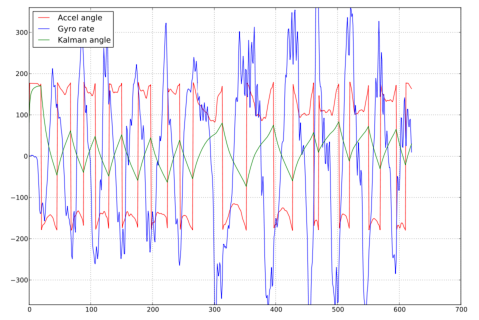
\includegraphics[scale=0.8]{fig/kalman_highfreq.pdf}
\caption{Kalman filter : High frequency input}
\label{fig:5_kalman_highfreq}
\end{figure}
Fig. \ref{fig:5_kalman_highfreq} has been plotted for a very high frequency movement of the IMU. As shown, the rates exceed 
$\pm320^o/s$ which is the maximum rate detected by the gyro. The final output of the kalman filter does match the hand movement
of about 90 degrees. However, at about the $300^{th}$ update, it completely misses a very fast 360 deg. rotation of the IMU. This
is reasonable because even the accelerometer and gyroscope do not seem to significantly register this movement.

\begin{figure}[!h]
\centering
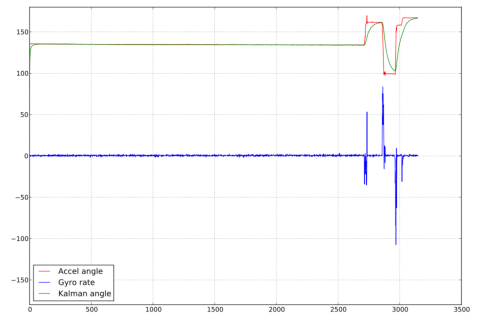
\includegraphics[scale=0.8]{fig/kalman_drift.pdf}
\caption{Kalman filter : Gyro drift}
\label{fig:5_kalman_gyrodrift}
\end{figure}
\newpage
Fig. \ref{fig:5_kalman_gyrodrift} shows readings plotted for 5 minutes at a 10 Hz update rate for the filter. It is seen that the
gyro rate has some noise. However, integrating this noise does not show a large error in the angle moved by the sensor. The
integral of the gyro rate is zero for all the time. The drift mentioned for gyroscopes is not to be seen even for periods as large as
12 minutes.

% \section{Motor Characteristics}
% We can look at the equations of a DC motor based on the electric model.\\
% \begin{tabular}{l@{ : }l}
%     $L$ & Inductance of the motor armature coil \\
%     $i$ & Instantaneous armature current \\
%     $V$ & Voltage applied at the coils \\
%     $e_b$ & Back EMF generated by the coils \\
%     $R_a$ & Armature resistance \\
%     $\tau$ & Net torque \\
%     $J_s$ & Moment of inertia of the motor shaft
% \end{tabular}
% \vspace{0.2in}
% 
% The electrical and mechanical system equations are as follows,
% \begin{eqnarray}
% L\frac{di}{dt} &=& V - iR_a - e_b \\
% J_s\frac{d\omega}{dt} &=& \tau
% \label{eqn:5_motoreqns}
% \end{eqnarray}
% 
% Electro-mechanical coupling constants for a DC motor. The torque constant results in $\tau = k_M\:i$ while the speed constant gives
% $e_b = k_E\:\omega_s$. These relations have been used in the simulations to get an idea of the extra torque available at a particular speed.
% 
% Assuming $L$ to be negligible, we get the following coupled equation as,
% \begin{equation}
% \tau = \frac{nk_M}{R_a}V - \frac{n^2k_Ek_M}{R_a}\:\omega
% \label{eqn:5_torqvolt}
% \end{equation}
% From Eqn. \ref{eqn:5_torqvolt}, we can see that the initial starting torque of a motor is large and decreases with increasing $\omega$. This also results in a large starting current for the motor from Eqn. \ref{eqn:5_motoreqns}. If we directly apply a constant voltage, the motor will take time to reach equilibrium. This time will be dependant on the load. To avoid this, we introduce
% a velocity control loop (PID) to obtain a trapezoidal profile. The results for a Maxon Amax motor with 16 cpr encoder and a 19:1
% gearbox running without any load are shown in Fig. \ref{fig:5_motorpid}
% \begin{figure}[!h]
% \centering
% 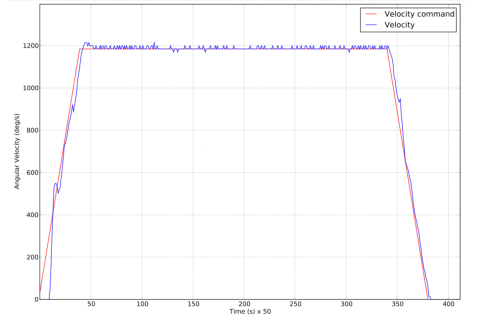
\includegraphics[scale=1.25]{fig/motor_pid.pdf}
% \caption{Motor velocity control}
% \label{fig:5_motorpid}
% \end{figure}






